\subsection{Overview}
% High-level components and their interaction
% TODO: @Hrvoje
\subsection{Component view}
% TODO: @Ozan
% Component diagram combining all components and each component having it's subcomponents in a different diagram with explanations
\subsection{Deployment view}
% TODO: @Roberto
% Deployment diagram with explaining each tier

The following diagram illustrates the physical architecture and the
deployment of the system.
Each node represents a piece of hardware which harbours one or more software units.
Each piece of hardware could be replicated multiple times to improve performances as  specified in later in this document.

\begin{figure}[H]
    \centering
    \hspace*{-3.5cm}
    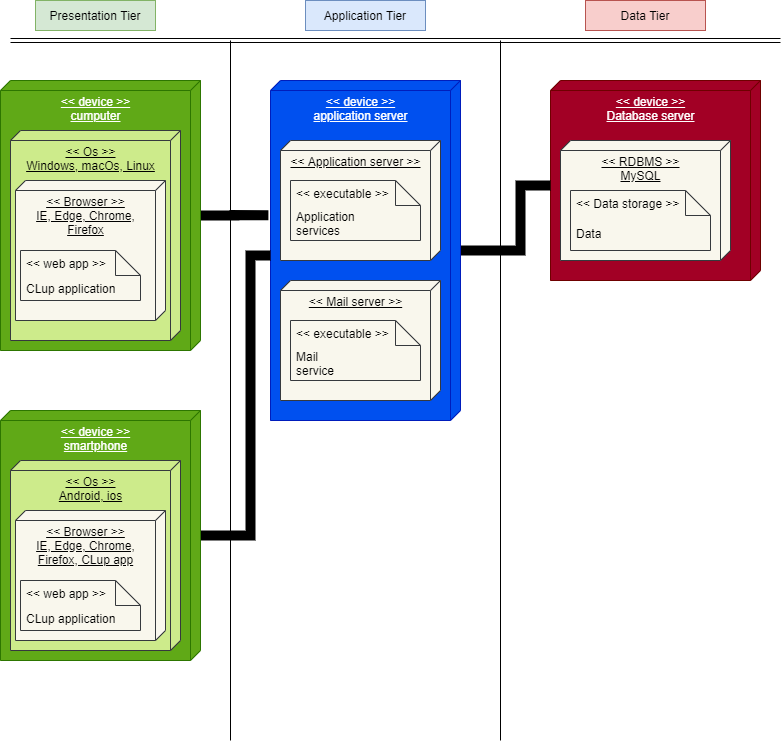
\includegraphics[height=0.7\textwidth]{Images/TierDiagram.png}
    \caption{World 1}
\end{figure}

As shown by the diagram, this system is deployed in a three-tier
architecture, where the three tiers consist of: \\
- Presentation tier is the highest-level tier and harbours the presentation logic.
The application is thought to be a web app, so it's accessible from every device with a browser, but it's probable that
a smartphone should be the most used device to access the application so there will be android and ios applications to access
the web app.
The smartphones applications will be more similar to a browser than to a real application.
In this tier there will not be application logic, so the architecture should be thin-client.
The only data stored on this tier is the jwt used for authentication. \\
- Application tier is the core level from the standpoint of logical management of the application services.
This tier contains all the application logic, from the scheduling of the line numbers to the managment of the store.
This tier is connected to the presentation tier through APIs.
An API is used for each action of the user, and the APIs are divided based on the role of the user.
Each user needs to authenticate using an API and reciving a jwt that needs to be attached to every subsequent request from the same user.
The jwt attached to the request is used to determine wich API are exposed to that user.
This tier contains also a mail Server to notify the users in case their line number is cancelled. \\

- Data tier ( tier 1 in the diagram) is the lowest-level tier as it contains all the information required to fuel the
application services, most prominently the query manager. The
databases are thought to be managed through an RDBMS
(Relational Database Management System), in particular MySQL. Relational databases
have the advantage of having near-maximum information density.
Relational constraints can improve the quality and
integrity of the content of the database.

\subsection{Runtime view}
% You can use sequence diagrams to describe the way components interact to accomplish specific tasks typically related to your use cases

% Main use cases with sequence diagrams indicating relations of each diagram to one another.

\subsection{Component interfaces}

% Class diagram with only methods demonstrating how components interact with each other.
% Also an ER or Class diagram to indicate data.
\subsection{Selected architectural styles and patterns}
% Please explain which styles/patterns you used, why, and how
\subsection{Other design decisions}

